\documentclass{article}

\usepackage{fancyhdr}
\usepackage{extramarks}
\usepackage[fleqn]{amsmath}
\usepackage{amsthm}
\usepackage{amsfonts}
\usepackage{tikz}
\usepackage[plain]{algorithm}
\usepackage{algpseudocode}
\usepackage{graphicx}
\usepackage{gensymb}
\usepackage{hyperref}

\DeclareRobustCommand{\bbone}{\text{\usefont{U}{bbold}{m}{n}1}}

\DeclareMathOperator{\EX}{\mathbb{E}}% expected value

\graphicspath{{./images/}}

\usetikzlibrary{automata,positioning}

%
% Basic Document Settings
%

\topmargin=-0.45in
\evensidemargin=0in
\oddsidemargin=0in
\textwidth=6.5in
\textheight=9.0in
\headsep=0.25in

\linespread{1.1}

\pagestyle{fancy}
\lhead{\hmwkAuthorName}
\chead{\hmwkClassShort\ \hmwkTitle}
\rhead{\firstxmark}
\lfoot{\lastxmark}
\cfoot{\thepage}

\renewcommand\headrulewidth{0.4pt}
\renewcommand\footrulewidth{0.4pt}

\setlength\parindent{0pt}

%
% Create Problem Sections
%

\newcommand{\enterProblemHeader}[1]{
    \nobreak\extramarks{}{Problem {#1} continued on next page\ldots}\nobreak{}
    \nobreak\extramarks{{#1} (continued)}{{#1} continued on next page\ldots}\nobreak{}
}

\newcommand{\exitProblemHeader}[1]{
    \nobreak\extramarks{{#1} (continued)}{{#1} continued on next page\ldots}\nobreak{}
    % \stepcounter{#1}
    \nobreak\extramarks{{#1}}{}\nobreak{}
}

\setcounter{secnumdepth}{0}
\newcounter{partCounter}

\newcommand{\problemNumber}{0.0}

\newenvironment{homeworkProblem}[1][-1]{
    \renewcommand{\problemNumber}{{#1}}
    \section{\problemNumber}
    \setcounter{partCounter}{1}
    \enterProblemHeader{\problemNumber}
}{
    \exitProblemHeader{\problemNumber}
}

%
% Homework Details
%   - Title
%   - Class
%   - Author
%

\newcommand{\hmwkTitle}{Midterm Exam}
\newcommand{\hmwkClassShort}{RBE 595}
\newcommand{\hmwkClass}{RBE 595 --- Reinforcement Learning}
\newcommand{\hmwkAuthorName}{\textbf{Arjan Gupta}}

%
% Title Page
%

\title{
    \vspace{2in}
    \textmd{\textbf{\hmwkClass}}\\
    \textmd{\textbf{\hmwkTitle}}\\
    \vspace{3in}
}

\author{\hmwkAuthorName}
\date{}

\renewcommand{\part}[1]{\textbf{\large Part \Alph{partCounter}}\stepcounter{partCounter}\\}

%
% Various Helper Commands
%

% Useful for algorithms
\newcommand{\alg}[1]{\textsc{\bfseries \footnotesize #1}}

% For derivatives
\newcommand{\deriv}[2]{\frac{\mathrm{d}}{\mathrm{d}#2} \left(#1\right)}

% For compact derivatives
\newcommand{\derivcomp}[2]{\frac{\mathrm{d}#1}{\mathrm{d}#2}}

% For partial derivatives
\newcommand{\pderiv}[2]{\frac{\partial}{\partial #2} \left(#1\right)}

% For compact partial derivatives
\newcommand{\pderivcomp}[2]{\frac{\partial #1}{\partial #2}}

% Integral dx
\newcommand{\dx}{\mathrm{d}x}

% Alias for the Solution section header
\newcommand{\solution}{\textbf{\large Solution}}

% Probability commands: Expectation, Variance, Covariance, Bias
\newcommand{\E}{\mathrm{E}}
\newcommand{\Var}{\mathrm{Var}}
\newcommand{\Cov}{\mathrm{Cov}}
\newcommand{\Bias}{\mathrm{Bias}}

\begin{document}

\maketitle

\nobreak\extramarks{Problem 1}{}\nobreak{}

\pagebreak

\begin{homeworkProblem}[Problem 1]
    Consider two random variables with distributions below:

    \[
        p = \{0.2, 0.2, 0.2, 0.2, 0.1, 0.1\}
    \]
    \[
        q = \{0.75, 0.0625, 0.0625, 0.0625, 0.0625\} 
    \]

    \begin{figure}[h!]
        \centering
        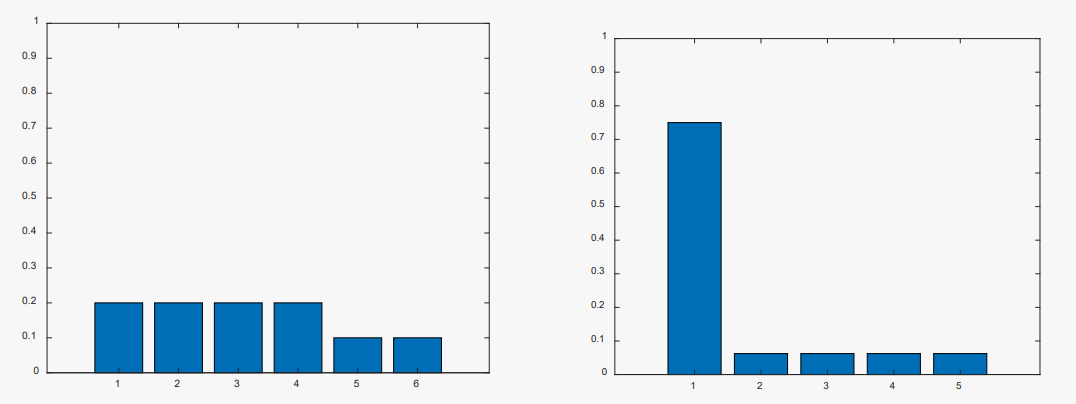
\includegraphics[scale=0.3]{prob1_histos.png}
    \end{figure}

    A. [4 points] Calculate the entropy for each variable.\\
    B. [4 points] Intuitively how can you tell which variable has a higher entropy without
    calculating the entropy numerically? What does higher entropy mean?

    \subsection{Answer}

    A. The entropy for each variable is given by:

    \begin{align*}
        H(p) &= -\sum_{i=1}^6 p_i \log_2 p_i \\
        &= -\left( 0.2 \log_2 0.2 + 0.2 \log_2 0.2 + 0.2 \log_2 0.2 + 0.2 \log_2 0.2 + 0.1 \log_2 0.1 + 0.1 \log_2 0.1 \right) \\
        &= -(4*0.2 \log_2 0.2 + 2*0.1 \log_2 0.1) \\
        &= 2.5219
    \end{align*}

    {\setlength{\mathindent}{1cm}
    \begin{align*}
        H(q) &= -\sum_{i=1}^5 q_i \log_2 q_i \\
        &= -\left( 0.75 \log_2 0.75 + 4*0.0625 \log_2 0.0625 \right) \\
        &= 1.3112
    \end{align*}}

    B. Entropy is defined as the lack of expected information, or the 
    `surprise'/uncertainty of a random variable. 
    We can tell that $q$ has a higher entropy than $p$ without calculating the entropy,
    because the histogram for $q$ shows that there is a `surprising' value of 0.75, which
    goes against the trend of the other values (which are all 0.0625). On the other hand,
    the histogram for $p$ shows that all the values are fairly close to each other. In general,
    higher entropy means that the random variable has more uncertainty,
    so the likelihood of encountering a value closer to the expected value is lower.



\end{homeworkProblem}

\nobreak\extramarks{Problem 2}{}\nobreak{}

\pagebreak

\begin{homeworkProblem}[Problem 2]
    \begin{figure}[h!]
        \centering
        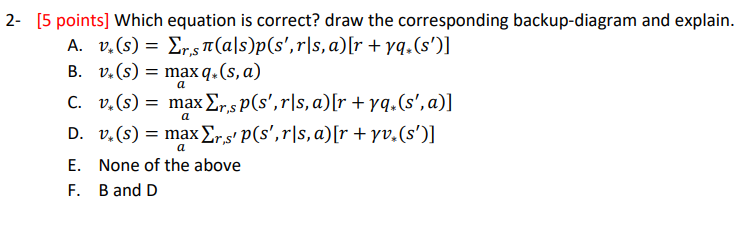
\includegraphics[scale=0.5]{prob2_prompt.png}
    \end{figure}

    \subsection{Answer}

    Option F (B and D) is correct.\\

    I have drawn the backup diagram for $v_*$ as given below:

    \begin{figure}[h!]
        \centering
        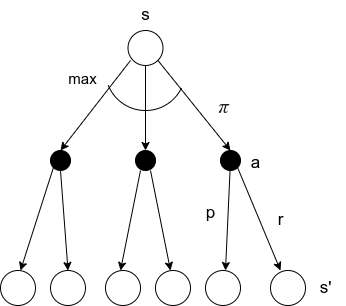
\includegraphics[scale=0.5]{vstar_drawio.png}
    \end{figure}

    \textbf{Explanation}

    $v_*$ is the optimal state-value function. The backup diagram for $v_*$ shows us that,
    if we start at a state s, we choose the action that maximizes the value of the state-action
    pair, and then we take the action. The action choice is taken using our current policy,
    $\pi$. Once we take the action, we end up in a new state, $s'$, and we get a reward, $r$.
    The resultant state $s'$ as well as the reward $r$ are chosen according
    to the dynamics of the environment, $p(s', r | s, a)$, which is not something we can control.
    In summary, the optimal state value function chooses the action that maximizes the value
    of the state-action value.\\

\end{homeworkProblem}

\nobreak\extramarks{Problem 2}{}\nobreak{}

\pagebreak

\nobreak\extramarks{Problem 3}{}\nobreak{}

\begin{homeworkProblem}[Problem 3]
    Consider a vehicle with 4 actions (left, right, up, down). There's no uncertainty in the outcome
    of the action (i.e. when left is commanded, the left state is achieved). The actions that cause
    the vehicle outside the grid, leave the state unchanged.
    The reward for all transition is -1 except when the goal is reached where the reward is zero.
    Discount factor $\gamma = 1$.\\
    The figure on left shows the name of the states and figure on the right shows the state-value
    $V(s)$, for each state under a uniform random policy.

    \begin{figure}[h!]
        \centering
        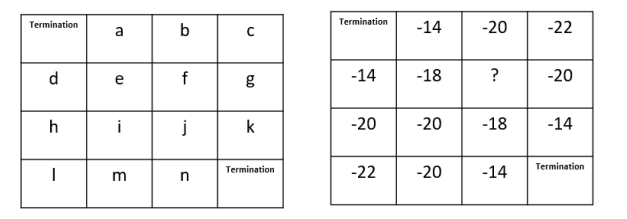
\includegraphics[scale=0.5]{prob3_prompt.png}
    \end{figure}

    A. [4 points] What is $q(k, down)$?\\
    B. [4 points] What is $q(g, down)$?\\
    C. [4 points] What is $V(f)$?\\

    \subsection{Answer}

    \textbf{A.} We know the equation for $q(s, a)$ is given by,

    \begin{align*}
        q(s, a) &= \sum_{s', r} p(s', r | s, a) \left[ r + \gamma V(s') \right]
    \end{align*}

    We can calculate $q(k, down)$ as follows:

    \begin{align*}
        q(k, down) &= \sum_{s', r} p(s', r | k, down) \left[ r + \gamma V(s') \right] \\
        &= 1 \left[ 0 + 1 \cdot 0 \right]\\
        &= 0
    \end{align*}

    \textbf{B.} We can calculate $q(g, down)$ as follows:

    \begin{align*}
        q(g, down) &= \sum_{s', r} p(s', r | g, down) \left[ r + \gamma V(s') \right] \\
        &= 1 \left[ -1 + 1 \cdot -14 \right]\\
        &= -15
    \end{align*}

    \textbf{C.} We know the equation for $V(s)$ is given by,

    \begin{align*}
        V(s) &= \sum_{a} \pi(a | s) q(s, a)
    \end{align*}
    
    We can calculate $V(f)$ as follows:

    \begin{align*}
        V(f) &= \sum_{s', r} p(s', r | f, \pi(f)) \left[ r + \gamma V(s') \right] \\
        &= 0.25 \left[ -1 + 1 \cdot -18 \right] + 0.25 \left[ -1 + 1 \cdot -20 \right] + 0.25 \left[ -1 + 1 \cdot -20 \right] + 0.25 \left[ -1 + 1 \cdot -18 \right]\\
        &= 0.25 \left[ -19 \right] + 0.25 \left[ -21 \right] + 0.25 \left[ -21 \right] + 0.25 \left[ -19 \right]\\
        &= 0.25 \left[ -80 \right]\\
        &= -20
    \end{align*}
    
\end{homeworkProblem}

\pagebreak

\nobreak\extramarks{Problem 4}{}\nobreak{}

\begin{homeworkProblem}[Problem 4]
    \begin{figure}[h!]
        \centering
        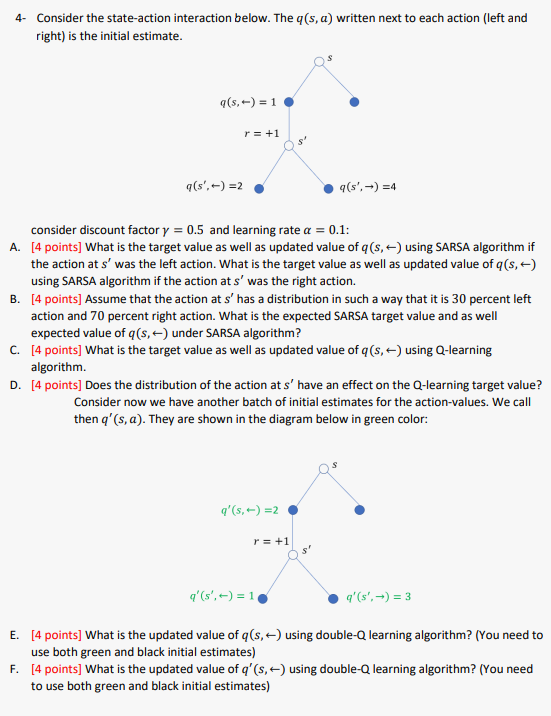
\includegraphics[scale=0.8]{prob4_prompt.png}
    \end{figure}

    \subsection{Answer}

    \textbf{A.} The target value for SARSA is given by
    $R_{t+1} + \gamma Q(S_{t+1}, A_{t+1})$.\\
    The update rule for SARSA is given by $Q(S_t, A_t) \leftarrow Q(S_t, A_t) + \alpha \left[ target - Q(S_t, A_t) \right]$.\\


    \textit{For left action at $s'$}:\\
    The target SARSA value at $q(s, left)$ is given by $1 + 0.5 \cdot 2 = 2$\\
    The update rule for SARSA is given by $1 + 0.1 \cdot (2 - 1) = 1.1$\\

    \textit{For right action at $s'$}:\\
    The target SARSA value at $q(s, right)$ is given by $1 + 0.5 \cdot 4 = 3$\\
    The update rule for SARSA is given by $1 + 0.1 \cdot (3 - 1) = 1.2$\\

\end{homeworkProblem}

\pagebreak

\nobreak\extramarks{Problem 5}{}\nobreak{}

\begin{homeworkProblem}[Problem 5]
    What are the 4 steps of the MCTS algorithm? How does MCTS balance exploration and
    exploitation?

    \subsection{Answer}

    The 4 steps of the MCTS algorithm are:

    \begin{enumerate}
        \item \textbf{Selection}: Starting from the root node, we select a leaf node
            with an exploration-exploitation trade-off criteria (UCB1).
        \item \textbf{Expansion}: We expand the leaf node by adding a child node for each
            possible action.
        \item \textbf{Simulation}: We simulate an episode starting from the newly added
            child node. We use the roll-out policy to select actions during the simulation.
        \item \textbf{Back-up}: We store action-values for each node in the tree.
    \end{enumerate}

    Specifically, in the selection step, for balancing exploration and exploitation, we use the UCB1 formula:

    \begin{align*}
        UCB1(S_i) = \frac{v_i}{n_i} + C \sqrt{\frac{\ln N_i}{n_i}}
    \end{align*}

    Where,\\
    $n_i$ is the number of times we have visited node $S_i$,\\
    $N_i$ is the number of times we have visited the parent of node $S_i$,\\
    $v_i$ is the value of node $S_i$, and\\
    $C$ is a constant that we choose.\\

    The flow chart for the MCTS algorithm (tree policy) is shown below:

    Now, let us describe how we use the above flow chart to balance exploration and exploitation.
    At first, we just have the root node, $S_0$. This technically currently a leaf node, but
    since it is the root-node, we make an exception and immediately add new child nodes to it,
    and rollout from the first new child node. Based on the results of the rollout, we update
    the value of the first new child node and its parent.\\

    Then, we restart the algorithm from the root node. This time, since the root node is no longer
    a leaf node, we need to use UCB1 to select a leaf node. Now this is where the exploration-exploitation
    trade-off comes in. We will find that even though the first new child node has a high value (since
    we rolled out from it previously), it would be the choice in case of greedy selection. However,
    since we are using UCB1, we will instead consider the second new child node, which has a lower value,
    because its exploration term is higher. Specifically, the exploration term is higher because $n_i$ is
    0, making the second term in the UCB1 for that node infinitely large. This shows that in the planning
    phase, MCTS balances exploration and exploitation by using the UCB1 formula.\\


\end{homeworkProblem}

\pagebreak

\nobreak\extramarks{Problem 6}{}\nobreak{}

\begin{homeworkProblem}[Problem 6]
    \textbf{(Exercise 8.1, page 166)} The nonplanning method looks particularly poor in Figure 8.3 because it is
    a one-step method; a method using multi-step bootstrapping would do better. Do you
    think one of the multi-step bootstrapping methods from Chapter 7 could do as well as
    the Dyna method? Explain why or why not.

    \subsection{Answer}

    Let us analyze how the $n$-step TD method would be applied to this problem.\\

    Firstly, in $n$-step TD, the $G_{t:t+n}$ is given as,

    \begin{align*}
        G_{t:t+n} = R_{t+1} + \gamma R_{t+2} + \ldots + \gamma^{n-1} R_{t+n} + \gamma^n Q(S_{t+n}, A_{t+n})
    \end{align*}

    One thing to notice is that, as given in the problem prompt, the reward for all actions
    is 0 except for the goal state, where the reward is 1. Therefore, we have two cases,
    depending on whether the goal state is reached within $n$ steps or not.\\

    If $t < T$, then $G_{t:t+n}$ is given as,

    \begin{align*}
        G_{t:t+n} &= 0.95^n Q(S_{t+n}, A_{t+n})
    \end{align*}

    If $t \geq T$, then $G_{t:t+n}$ is given as,

    \begin{align*}
        G_{t:t+n} &= 0.95^{k-1} + 0.95^k Q(S_{t+n}, A_{t+n})
    \end{align*}

    Where $k$ is the number of steps taken before reaching the goal state (i.e. $k = T - t$).\\

    And $Q(S_t, A_t)$ is given as,

    \begin{align*}
        Q(S_t, A_t) &= Q(S_t, A_t) + \alpha \left[ G_{t:t+n} - Q(S_t, A_t) \right]
    \end{align*}

    We can see that if we use 1-step TD, the algorithm's environment-interaction steps will
    be very similar to Dyna-Q with $n = 0$ planning steps.\\

    However, I believe that in this particular problem,
    \textbf{the general n-step TD method will not perform as well
    as n-planning step Dyna-Q}, because it will take longer than Dyna-Q to learn the state-action
    values of the states leading up to the goal state. This is because, initially the state-action
    values of all the states will be 0. Then,
    the n-step TD method will only update the value of the
    state-action pair that encounters the goal state. All the states leading up to the goal state
    will simply have their value updated to 0. After a few episodes, the state-action values
    will be updated to non-zero values, but it will take longer than Dyna-Q.\\

    On the other hand, Dyna-Q will use the simulated experience to update the value of all the
    state-action pairs that were encountered in the simulated experience. It will make good
    use of computational resources in its planning phase. With only 1 episode and a sufficiently
    large number of planning steps, Dyna-Q will be able to learn non-zero values for the
    state-action values leading up to the goal state.\\

    By the second or third episode, Dyna-Q will have learned the state-action values of the
    states leading up to the goal state much better than the n-step TD method. Perhaps after
    a high number of episodes, the n-step TD method will catch up to Dyna-Q, but it will
    be behind initially. Therefore,
    I think if we compare the general performance of the two algorithms for this particular problem,
    Dyna-Q will perform better than the n-step TD method.\\

\end{homeworkProblem}

\pagebreak

\nobreak\extramarks{Problem 7}{}\nobreak{}

\begin{homeworkProblem}[Problem 7]
    \textbf{(Exercise 8.2, page 168)} Why did the Dyna agent with exploration bonus, Dyna-Q+, perform
    better in the first phase as well as in the second phase of the blocking and shortcut
    experiments?

    \subsection{Answer}

    In the first phase, as described in Example 8.2, 
    the maze has an opening on the near side, and a wall on the far side.
    After 1000 time steps, the short path is blocked and the far side opening is created. The graph
    for the performance of Dyna-Q and Dyna-Q+ is shown below:

    We can see that Dyna-Q+ performs better than Dyna-Q before and after the 1,000 time step mark.
    Before the 1,000 time step mark, Dyna-Q+ performs better because it is able to explore the
    grid-world more than Dyna-Q. This is because Dyna-Q+ uses the exploration bonus in its planning
    phase, given by $R = r + \kappa \sqrt{\tau(s, a)}$. This encourages the agent to find the far
    edge faster than Dyna-Q. After the 1,000 time step mark, Dyna-Q+ performs better again for the
    same reason. Since the short path is blocked, Dyna-Q+ is able to explore the grid-world
    faster than Dyna-Q.\\

    In the second phase, as described in Example 8.3, the maze has an opening on far side,
    and after the 3,000 time step mark, the short path is additionally opened. The graph
    for the performance of Dyna-Q and Dyna-Q+ is shown below:

    While the performance of Dyna-Q+ and Dyna-Q is similar before the 3,000 time step mark,
    we can see that around roughly the 4,000 time step mark, Dyna-Q+ begins to perform
    noticeably better than Dyna-Q. Here, the reward bonus is helping Dyna-Q+ create
    trajectories that lead to the short path. This is because the reward bonus is given
    by $R = r + \kappa \sqrt{\tau(s, a)}$, where $\tau(s, a)$ is the number of time steps
    since the last visit to state $s$ after taking action $a$. Therefore, the reward bonus
    is higher for states that have not been visited in a long time. This encourages the
    agent to explore the grid-world more, and find the short path. The Dyna-Q agent does
    not have this advantage, and in fact never finds the short path, as noted by the book,
    ``even with an $\epsilon$-greedy policy, it is very
    unlikely that an agent will take so
    many exploratory actions as to discover the shortcut.'' So, exploration in the
    planning phase is what gives Dyna-Q+ the advantage over Dyna-Q.\\

\end{homeworkProblem}

\end{document}